\section{AML process}

\begin{figure}[h!]
  \begin{sequencediagram}
    \newinst{wallet}{\shortstack{Customer \\
      \\ 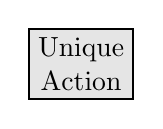
\begin{tikzpicture}
        \node [fill=gray!20,draw=black,thick,align=center] { Unique \\ Action};
      \end{tikzpicture}
    }}
    \newinst[2]{exchange}{\shortstack{Taler (exchange) \\
       \\ \begin{tikzpicture}[shape aspect=.5]
        \tikzset{every node/.style={cylinder,shape border rotate=90, draw,fill=gray!25}}
        \node at (1.5,0) {\shortstack{{{\tiny Database}}}};
       \end{tikzpicture}
    }}
    \newinst[2]{staff}{\shortstack{AML staff \\
      \\ 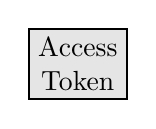
\begin{tikzpicture}
        \node [fill=gray!20,draw=black,thick,align=center] { Access \\ Token};
      \end{tikzpicture}
    }}
    \postlevel
    \mess[0]{wallet}{{Initial action}}{exchange}
    \begin{callself}{exchange}{Establish AML requirement}{}
    \end{callself}
    \begin{callself}{exchange}{Queue AML task}{}
    \end{callself}
    \mess[0]{exchange}{Wait for AML}{wallet}
    \mess[0]{staff}{Request AML work}{exchange}
    \mess[0]{exchange}{{Open AML task(s)}}{staff}
    \mess[0]{staff}{Request details}{exchange}
    \mess[0]{exchange}{KYC/AML data}{staff}
    \begin{callself}{staff}{Review and decide}{}
    \end{callself}
    \mess[0]{staff}{{Decision documentation}}{exchange}
    \mess[0]{exchange}{AML decision}{wallet}
    \mess[0]{wallet}{{Retry action}}{exchange}
\end{sequencediagram}
  \caption{Deposit interactions between customer, Taler exchange (payment
    service provider) and the AML staff.  The process can be
    triggered by various {\em actions} described in Chapter~\ref{chap:triggers}.
    AML staff interactions are cryptographically secured and
    decisions and the provided reasoning are archived by the exchange.
    AML staff may interact with the customer (out-of-band)
    in its decision process.
    }
  \label{fig:proc:aml}
\end{figure}
